\subsection{Intra-night Cadence}\label{q:Visits}

The Phase 1 recommendations relevant to the intra-night cadence were primarily focused on how pairs of visits should be acquired and the exposure time for individual visits. The SCOC recommended that visits in each pair should be acquired in different filters, enabling the measurement of color information for transients and variables on short time scales. Investigations by the scheduler team found that pairs of visits separated by $\sim33$ minutes resulted in the best balance between minimizing filter changes and maintaining a high fraction of visits acquired in pairs (\citeds{PSTN-053} Q5) that enable SSO trajectory recovery. 

The questions left open after the Phase 1 recommendations on intra-night cadence were: 

\begin{enumerate}
\item Should there be a third visit in a night? Should it be all the time or only on some nights?
\item Should a third nightly visit be added everywhere in the sky (as opposed to for example only or preferentially in the extragalactic \emph{vs} Galactic regions or based on Ecliptic Latitude)?
\item If there is going to be a third visit on a night, what should the spacing between the second and third visits be?
\item If there is no third visit, what should the time separation between visits in a pair be (\emph{e.g.} 33 minutes or 2-7 hours)?
\end{enumerate}

\subsubsection{SCOC recommendations: executive summary}\label{rec:intranight_es}

The SCOC recommends increasing the number of field revisits on time scales of hours-to-one-day. Overall, these time scales are generally not well sampled by ``classic'' LSST cadences (see \citealt{2019PASP..131f8002B,2022ApJS..258...13B, 2022ApJS..258....2L}), yet they are important in the discovery and characterization of transients, as well as being largely unexplored by other surveys, especially at high redshift, and thus covering them increases the discovery potential of LSST.

Simulations that increase the number of visits on these time scales include the \texttt{presto\_color, long\_gaps}, and \texttt{suppress\_repeat} families. The \texttt{presto\_color} family includes a third visit to each field in the same night. The original implementation did not control the third visit time gap, and telescope efficiency considerations caused it to be taken in short time intervals. In \opsim\ v2.1, this parameter is controlled and visits are spread out by as little as 1.5 hours and as much as 4 hours. Note that the original paper proposing a presto-color-like cadence \citep{2019PASP..131f8002B}\footnote{Originally submitted as a white paper in response to the 2018 Cadence White Papers call.} did \emph{not} recommend revisits on time scales $<4$ hours as those time scales are too short to meaningfully constrain flux evolution even for (known) rapidly evolving transients, thus the scientific benefit of this family of simulations is not clear. Nonetheless, this family of simulations with an increasing time gap for the third visit reveals important trends in response to the addition of a third visit which we discuss in the next paragraph. The \texttt{long\_gaps} family of simulations implements repeat visits on longer time scales, implemented both in visit triplets and in pairs of visits (\emph{i.e.} separating the pair by several hours).
An additional relevant family of simulations is the \texttt{suppress\_repeat} which actively suppresses the third visit in a night. By preventing the scheduler from taking these third visits it forces it instead to take other less-preferred observations, including fields that were observed on the immediately prior night. Thus this family further undersamples the timescale between 33 minutes and 12 hours, but increases the sampling at $\sim$24 hours. Finally, it should be noted that the implementation of a rolling cadence also helps reduce the minimum revisit time gap and increases the number of images that fall into the hours-to-one-day time scales.


Scientific metrics that are sensitive to these cadences include the kilonova metrics, as well as metrics designed to detect rare and unusual phenomena (Presto- and Presto-Color metrics, not to be confused with the \texttt{presto-color} family of simulations). Generally, we found all these metrics benefit from the inclusion of a third visit and to steadily improve as the time gap is increased up to several hours or into the following night. However, including a third visit to the same field within a night has an impact on survey efficiency because it adds a constraint on the selection of target fields that may take precedence over image quality and slew time considerations. Thus most metrics sensitive to image quality or to the number of images collected are negatively affected if third visits in the same night are required extensively. For example, many SSSC metrics including detection fractions and light curve inversion metrics for the different Solar System populations
 perform poorly on the \texttt{presto\_color} family of simulations, especially when the time gaps are short and the constraints on field selection are tighter. In addition to these specific scientific metrics, the TimeGaps metric (\autoref{fig:tgaps}) provides a science-case-agnostic gauge of the number of revisits that fall in this range of revisit timescales.


{\bf With these considerations, the SCOC converged on recommending that visit are paired with the visits in the pair spaced by $\sim33$ minutes, taken with different filters, as implemented in the \texttt{baseline\_v2.0} and most v2.X simulation (see \autoref{sec:v3} for details on the band pairing, which may be subject to further study).
This time spacing is critical for Solar System science, and the different filters provide a color measurement useful for transient characterization. Further, the SCOC recommends the LSST cadence be designed to ensure coverage of time scales in the hours-to-one-day range by carefully tuning survey parameters in combination. Performing three visits per night by default is not recommended, but a combination of preferentially pushing a third visit to the following night (which can be achieved by implementing a rolling cadence, see \autoref{q:Rolling}, in conjunction with the suppression of a third nightly visit as done in the \texttt{suppress\_repeat} family of simulations) and requesting a third visit within a night once every several nights ($\sim1$ week) would achieve this goal.
It is important these third visits be taken in one of the bands that were already observed in the paired visits.}

It is hard to better quantify at this time the precise amount of time or number of visits that should be spent on the hours-to-one-day revisit time scales. The discovery potential in this region is obvious and driven by the fact that these time scales are currently poorly explored, particularly at the high redshifts that LSST will reach. The investment in these time scales should be reevaluated regularly throughout the survey. 

We further note that, while a third visit during the same night can plausibly be a single visit (i.e. not a pair separated by 33 minutes), next-night observations may need to be paired to preserve the ability to use the visits for linking Solar System objects (\emph{i.e.} third and fourth visits).

\subsubsection{SCOC recommendations: point by point answers}\label{rec:intranight}

\begin{enumerate}

\item The third visit within the same night should be implemented for only a small fraction of observing time. The SCOC tentatively suggests implementing third visits for one night out of every 7 nights, but this could also be distributed in other ways at a similar total time fraction (see also \autoref{q:Rolling}).

\item Since the scientific motivation for the implementation of the third visit is broad and includes the discovery of unknown, unexpected phenomena, there is no strong motivation to limit the third visit to some areas of the sky. But we note that the SCOC has suggested specific exploration of survey parameters, such as footprint and filter selection, that would enhance Galactic science (see \autoref{q:Footprint} and \autoref{q:Filters} ). \emph{Similarly, if Galactic science can demonstrably be enhanced by a different intra-night cadence this recommendation may change outside of the low-dust WFD footprint}.


\item Because a goal of having three visits in one night is to ensure coverage of a phenomenon over a range of timescales, we recommend that third nightly visits be broadly distributed in the 2-7 hour range rather than on a rigid cadence.
We also encourage some small fraction of revisits on the immediately following night, to further improve measurements on timescales faster than three days.
This is consistent with the recommendations from several cadence notes (\citealt{2022ApJS..258...13B},\footnote{\url{https://docushare.lsst.org/docushare/dsweb/Get/Document-37644/Delta_T_2021.pdf}.} \citealt{2022ApJS..258....2L},\footnote{\url{https://docushare.lsst.org/docushare/dsweb/Get/Document-37653/Anomalies.pdf}.}, and Richards et al. 2019\footnote{\url{https://docushare.lsstcorp.org/docushare/dsweb/Get/Document-30572/richards_agn_rolling_wfd.pdf}.} as well as \citealt{2019PASP..131f8002B}.


\item 
The science goal of many of the third-visit proposals is to obtain both a color and a rate of change, and increasing the time separation of the two visits in a pair is insufficient to meet these requests.
The revisit time within pairs was already addressed in the SCOC Phase 1 recommendations. Thus the SCOC recommends that the visit are paired as designed in the v2.X simulations with a goal of $\sim33$ minutes separation.


\end{enumerate}
\begin{figure}
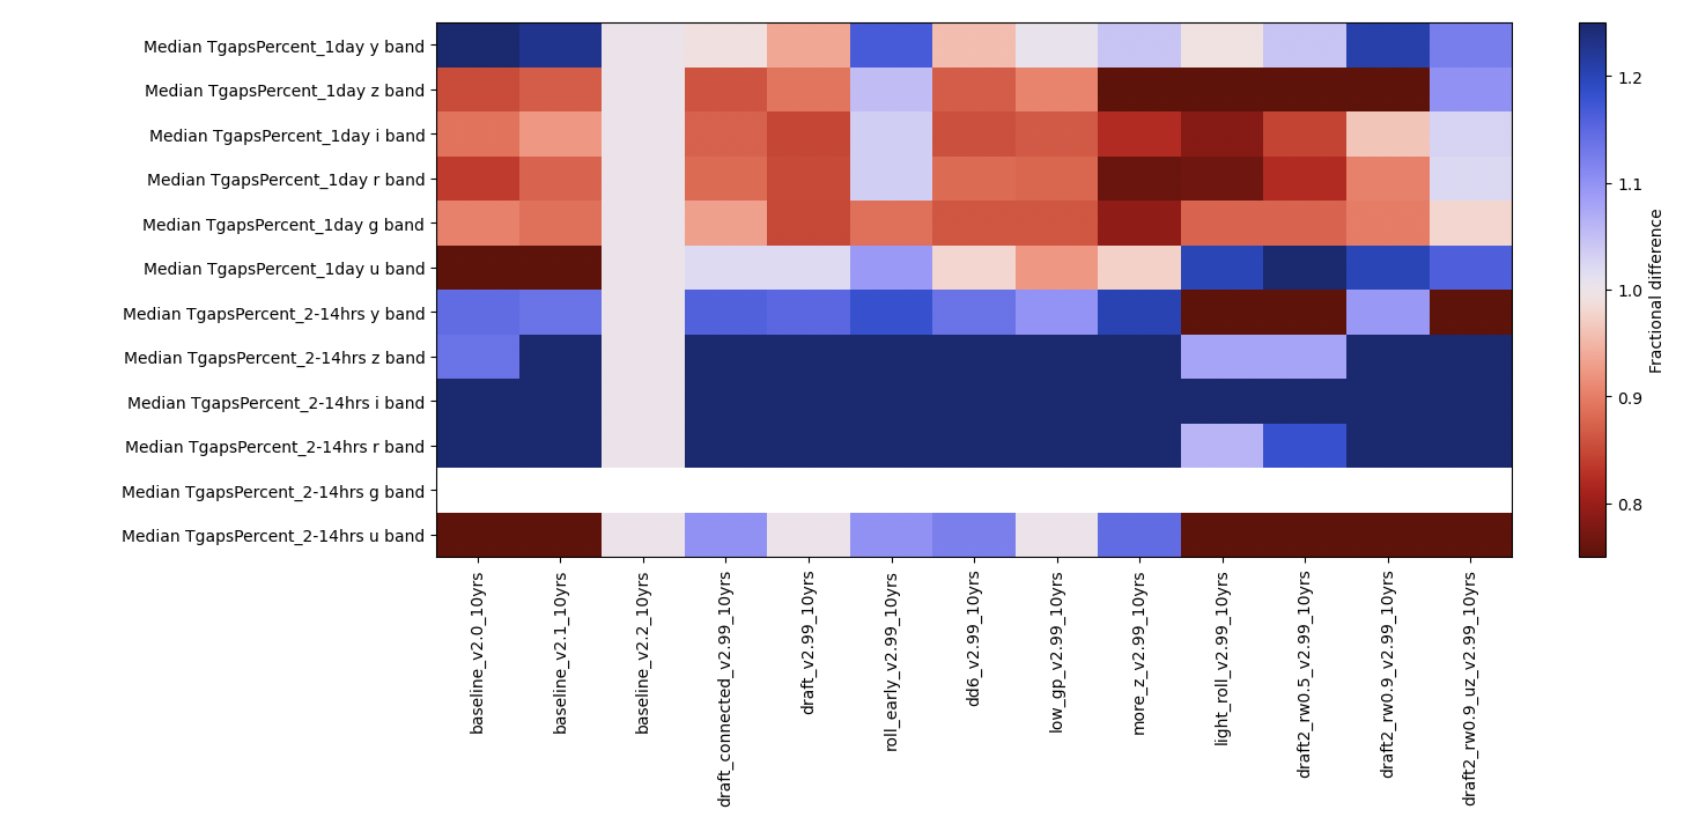
\includegraphics[width=0.95\textwidth, right]{figures/tgaps.png}
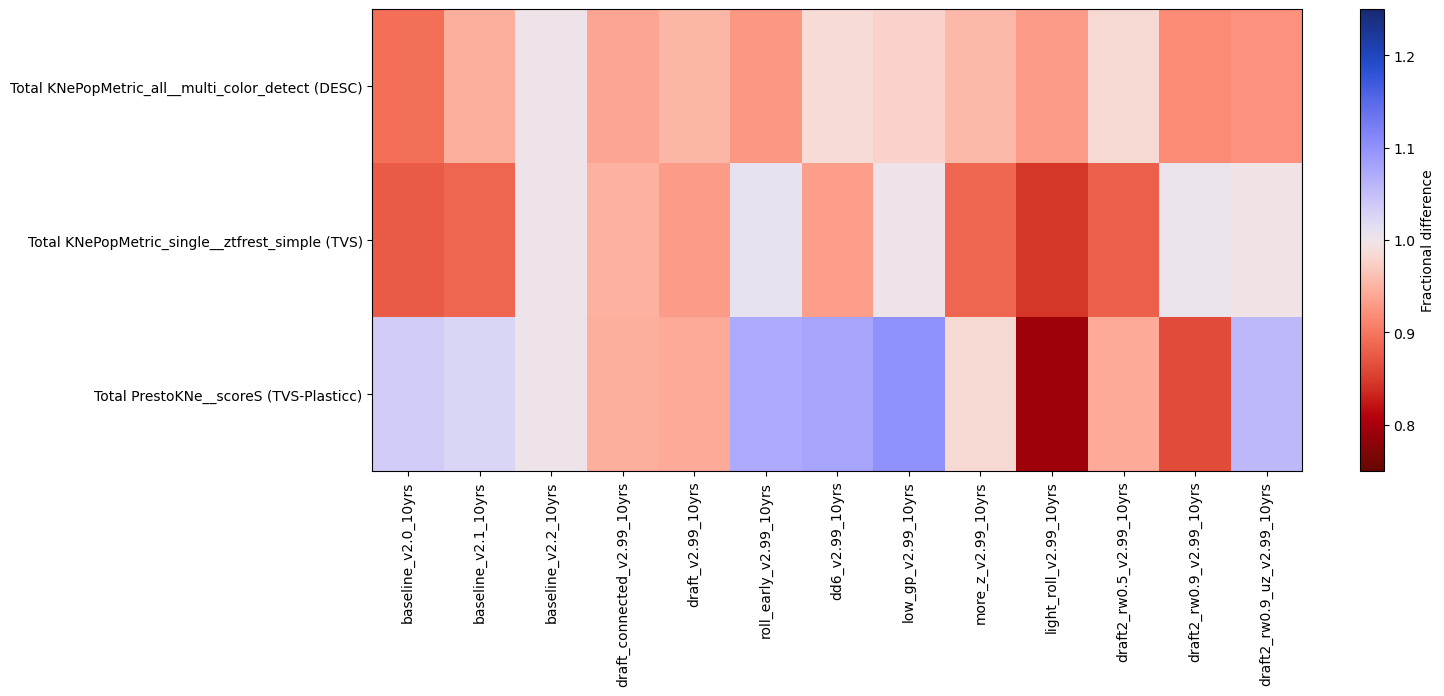
\includegraphics[width=0.94\textwidth, right]{figures/kne.png}
\caption{The response of metrics sensitive to intra-night cadence to the v2.X baselines and the v2.99 simulations. The performance is benchmarked in both plots with respect to \texttt{baseline\_v2.2}. Top: metrics showing the fraction of visits falling in the 2-14 hours and one day time ranges for different filters; bottom: three kilonovae metrics. Note: the simulation appearing here as \texttt{draft\_rw0.9\_uz\_v2.99\_10yrs} was subsequently adopted as \texttt{baseline\_v3.0}.}
\label{fig:tgaps}
\end{figure}

A final point should be made about the relationship between the time-gap distribution and the filter exchanges. As noted in \autoref{q:Filters}, the Rubin filter wheel can host 5 of the 6 filters on any given night. Which filters should be swapped and when is under discussion and some science cases (SN Ia cosmology in particular) benefit from increased access to some bands (\emph{e.g.} $z$) to reduce time gaps between sets of observations (particularly in the DDFs, \autoref{q:DDF}). However, the choice of filters on the wheel impacts more than the specific filters that are involved in the swap, due to the prescribed pairing of filters for the observation pairs, themselves driven by efficiency considerations including pairing filters suited to observe under similar conditions and enhancing the discoverability of SSOs (see \autoref{sec:v3}). \emph{As indicated in \autoref{q:Filters}, the filter swapping strategies deserve more attention, and we recommend that the impact of these choices on time gaps in all filters be monitored when alternative filter change strategies are tested in simulations}.
